%# -*- coding: utf-8-unix -*-
% !TeX spellcheck = zh_CN
\documentclass[oneside,UTF8,a4paper,12pt]{book}		% twoside 表示双面打印

\usepackage{url}
\usepackage{cite}
\usepackage{color}
\usepackage{xcolor}
\usepackage{import}
\usepackage{hyperref}								% 添加超链接
\usepackage{graphicx}
\usepackage{enumitem}
\usepackage{listings}								% 代码
\usepackage{transparent}
\usepackage{indentfirst}							% 段首缩进
\usepackage{supertabular}							% 长表格(换页处理)
\usepackage[utf8]{inputenc}
%\usepackage[hyphenbreaks]{breakurl}					% 超链接自动换行


\graphicspath{{./img/}}

\setlength{\parindent}{2em}							% 段首缩进
\setlength{\parskip}{1em}							% 段落间距
\renewcommand{\baselinestretch}{1.5}				% 行间距

% 自定义命令

% 设置itemize行间距
\setitemize{
	itemsep=0pt,
	partopsep=0pt,
	parsep=0.8em,
	topsep=5pt}
	
% 代码颜色设置
\lstset{ 
	backgroundcolor=\color{white},   				% 选择代码背景,必须加上\ usepackage {color}或\ usepackage {xcolor}.
	basicstyle=\footnotesize,        				% 设置代码字号.
	breakatwhitespace=false,         				% 设置是否当且仅当在空白处自动中断.
	breaklines=true,                 				% 设置自动断行.
	captionpos=b,                    				% 设置标题位置.
	commentstyle=\color{mygreen},    				% 设置注释格式
	deletekeywords={...},            				% 是否删除给定语言的关键词.
	escapeinside={\%*}{*)},          				% 是否在代码中添加LaTex.
	extendedchars=true,              				% 是否允许使用非ASCII字符; 仅适用于8位编码,不适用于UTF-8. 
	frame=single,	                   				% 给代码区添加边框.
	keepspaces=true,                 				% 保留空格(useful for keeping indentation of code (possibly needs columns=flexible).
	keywordstyle=\color{blue},       				% 关键字显示风格.
	morekeywords={*,...},            				% 是否需要添加其他的关键词.
	numbers=left,                    				% 给代码添加行号,可取值none, left, right.
	numbersep=5pt,                   				% 设置行号与代码之间的间隔
	numberstyle=\tiny\color{green}, 				% 行号的字号和颜色
	rulecolor=\color{black},         				% 边框颜色,如果没有设置,框架颜色可以在非黑色文本中的换行符上更改(例如 text (e.g. comments (green here)))
	showspaces=false,                				% 显示每个地方添加特定下划线的空格; 覆盖了'showtringspaces'
	showstringspaces=false,          				% 仅在字符串中允许空格
	showtabs=false,                  				% show tabs within strings adding particular underscores
	stepnumber=1,                    				% the step between two line-numbers. If it's 1, each line will be numbered
	stringstyle=\color{mymauve},     				% string literal style
	tabsize=4,	                   					% 将默认tab设置为2个空格
	title=\lstname                   				% show the filename of files included with \lstinputlisting; also try caption instead of title
}

% 定义
\newtheorem{note}{注意:}

% 去掉超链接红框
\hypersetup{hidelinks,
	colorlinks=true,
	allcolors=blue,
	pdfstartview=Fit,
	breaklinks=true}

\makeatletter
\def\UrlAlphabet{%
	\do\a\do\b\do\c\do\d\do\e\do\f\do\g\do\h\do\i\do\j%
	\do\k\do\l\do\m\do\n\do\o\do\p\do\q\do\r\do\s\do\t%
	\do\u\do\v\do\w\do\x\do\y\do\z\do\A\do\B\do\C\do\D%
	\do\E\do\F\do\G\do\H\do\I\do\J\do\K\do\L\do\M\do\N%
	\do\O\do\P\do\Q\do\R\do\S\do\T\do\U\do\V\do\W\do\X%
	\do\Y\do\Z}
\def\UrlDigits{\do\1\do\2\do\3\do\4\do\5\do\6\do\7\do\8\do\9\do\0}
\g@addto@macro{\UrlBreaks}{\UrlOrds}
\g@addto@macro{\UrlBreaks}{\UrlAlphabet}
\g@addto@macro{\UrlBreaks}{\UrlDigits}
\makeatother

% 字体
\usepackage{xeCJK}
\usepackage{graphicx}
\usepackage{fontspec} 
\setCJKmainfont{Source Han Mono SC} 


\begin{document}

\author{丁敬}
\title{X 教程}
\date{2023年04月26日}

\frontmatter										 % 对前言和概览用罗马数字作为页码
\mainmatter      		 							% 对正文用阿拉伯数字作为页码
\maketitle
\tableofcontents


\mainmatter
\chapter{新手开发者指南}

\section{X系统概念}

本章旨在向您介绍您需要了解的X窗口系统的基本概念和术语。当你有了这些概念,你将准备在后面的章节中更深入地研究特定的主题。

\subsection{X基于C/S结构}

X被设计成允许多个程序共享对一组公共硬件的访问。这种硬件既包括输入设备,如鼠标和键盘,也包括输出设备,如视频适配器和连接到它们的显示器。这些公共硬件由指定的某个进程进行统一管理,这个进程称为X服务端(因为它向客户机应用程序提供硬件设备的服务)。


与许多C/S系统一样,X服务端通常向许多同时运行的客户机提供服务,因此X服务端比大多数客户机运行的时间更长,并侦听来自新客户机的传入连接。


许多用户只在独立的笔记本电脑或桌面系统上使用X。在此设置中,X客户端与X服务器运行在同一台计算机上。然而,X为客户端/服务器通信定义了一个流协议。该协议可以通过网络公开,以允许客户端连接到不同机器上的服务器。这里需要注意的是,在这个模型中,客户机/服务器标签可能会令人困惑。此时在你面前的笔记本如果显示了远程机器客户端生成的图形,那么你当前的笔记本就是X服务端,生成图形的远程机器则是X客户端,如图 \ref{img-1.1.1-1}。


\begin{figure}[h]
    \centering
    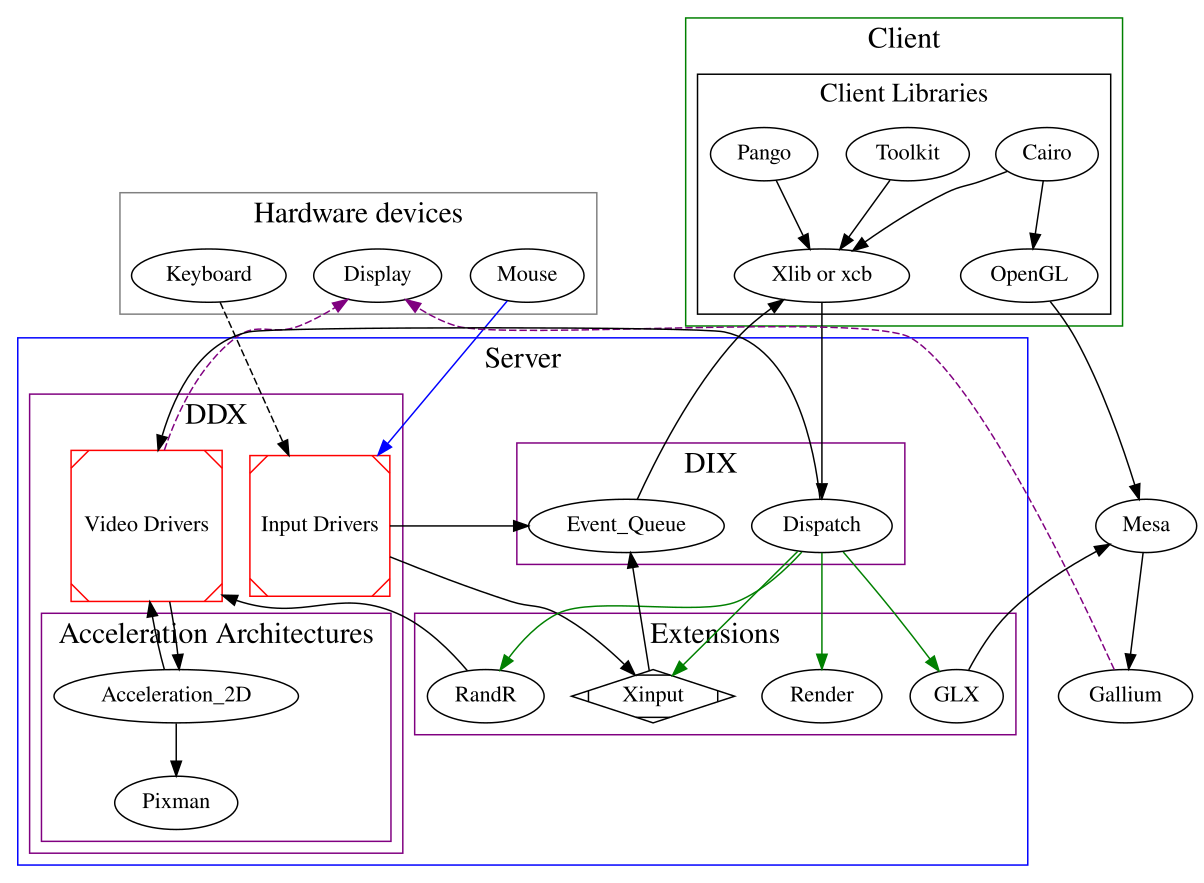
\includegraphics[scale=0.40]{x-1-1.png}
    \caption{X客户端/服务端模型}
    \label{img-1.1.1-1}
\end{figure}

\subsection{X实践}

本节描述X的一些基本组件及其工作原理。这个部分内容很多,有点像大杂烩。推荐的阅读方法是浏览一遍,然后回过头再读一遍。

\subsubsection{通过键盘输入}

X服务执行的任务之一是处理键盘上的输入,并将相应的键事件发送到适当的客户机应用程序。在简单的X配置中,每次只有一个客户端具有“输入焦点”,并且大多数关键事件将发送到该客户端。根据窗口管理器配置,只需将鼠标移动到另一个窗口、单击鼠标、使用热键或操作显示可用客户机的面板,就可以将焦点移动到另一个窗口。具有焦点的客户端通常以某种方式突出显示,以便用户可以知道他们的输入将流向何处。客户端可以使用“抓取”(在本章后面描述)来覆盖向重点客户端发送关键事件的默认交付。



\backmatter
% bibliography, glossary and index would go here.

\end{document}